\documentclass[12pt,letterpaper]{article}
\usepackage{graphicx,textcomp}
\usepackage{natbib}
\usepackage{setspace}
\usepackage{fullpage}
\usepackage{color}
\usepackage[reqno]{amsmath}
\usepackage{amsthm}
\usepackage{fancyvrb}
\usepackage{amssymb,enumerate}
\usepackage[all]{xy}
\usepackage{endnotes}
\usepackage{lscape}
\newtheorem{com}{Comment}
\usepackage{float}
\usepackage{hyperref}
\newtheorem{lem} {Lemma}
\newtheorem{prop}{Proposition}
\newtheorem{thm}{Theorem}
\newtheorem{defn}{Definition}
\newtheorem{cor}{Corollary}
\newtheorem{obs}{Observation}
\usepackage[compact]{titlesec}
\usepackage{dcolumn}
\usepackage{tikz}
\usetikzlibrary{arrows}
\usepackage{multirow}
\usepackage{xcolor}
\newcolumntype{.}{D{.}{.}{-1}}
\newcolumntype{d}[1]{D{.}{.}{#1}}
\definecolor{light-gray}{gray}{0.65}
\usepackage{url}
\usepackage{listings}
\usepackage{color}
\usepackage[utf8]{inputenc}
\usepackage{verbatim} % includes comment blocks

\definecolor{codegreen}{rgb}{0,0.6,0}
\definecolor{codegray}{rgb}{0.5,0.5,0.5}
\definecolor{codepurple}{rgb}{0.58,0,0.82}
\definecolor{backcolour}{rgb}{0.95,0.95,0.92}

\lstdefinestyle{mystyle}{
	backgroundcolor=\color{backcolour},
	commentstyle=\color{codegreen},
	keywordstyle=\color{magenta},
	numberstyle=\tiny\color{codegray},
	stringstyle=\color{codepurple},
	basicstyle=\footnotesize,
	breakatwhitespace=false,
	breaklines=true,
	captionpos=b,
	keepspaces=true,
	numbers=left,
	numbersep=5pt,
	showspaces=false,
	showstringspaces=false,
	showtabs=false,
	tabsize=2
}
\lstset{style=mystyle}
\newcommand{\Sref}[1]{Section~\ref{#1}}
\newtheorem{hyp}{Hypothesis}

\title{Applied Stats II - Problem Set 1}
\date{Due: February 12, 2023}
\author{Imelda Finn (22334657)}

\begin{document}
	\maketitle
\begin{comment}
	\section*{Instructions}
	\begin{itemize}
	\item Please show your work! You may lose points by simply writing in the answer. If the problem requires you to execute commands in \texttt{R}, please include the code you used to get your answers. Please also include the \texttt{.R} file that contains your code. If you are not sure if work needs to be shown for a particular problem, please ask.
\item Your homework should be submitted electronically on GitHub in \texttt{.pdf} form.
\item This problem set is due before 23:59 on Sunday February 19, 2023. No late assignments will be accepted.
	\end{itemize}

	\vspace{.25cm}
\end{comment}

	Code in \texttt{PS1\_ImeldaFinn.R}


\section*{Question 1}
\vspace{.25cm}
\noindent The Kolmogorov-Smirnov test uses cumulative distribution statistics to test the similarity of the empirical distribution of some observed data and a specified PDF, and serves as a goodness of fit test. The test statistic is created by:

$$D = \max_{i=1:n} \Big\{ \frac{i}{n}  - F_{(i)}, F_{(i)} - \frac{i-1}{n} \Big\}$$

\noindent where $F$ is the theoretical cumulative distribution of the distribution being tested and $F_{(i)}$ is the $i$th ordered value. Intuitively, the statistic takes the largest absolute difference between the two distribution functions across all $x$ values. Large values indicate dissimilarity and the rejection of the hypothesis that the empirical distribution matches the queried theoretical distribution. The p-value is calculated from the Kolmogorov-
Smirnoff CDF:

$$p(D \leq x) \frac{\sqrt {2\pi}}{x} \sum _{k=1}^{\infty }e^{-(2k-1)^{2}\pi ^{2}/(8x^{2})}$$


\noindent which generally requires approximation methods (see \href{https://core.ac.uk/download/pdf/25787785.pdf}{Marsaglia, Tsang, and Wang 2003}). This so-called non-parametric test (this label comes from the fact that the distribution of the test statistic does not depend on the distribution of the data being tested) performs poorly in small samples, but works well in a simulation environment. Write an \texttt{R} function that implements this test where the reference distribution is normal. Using \texttt{R} generate 1,000 Cauchy random variables (\texttt{rcauchy(1000, location = 0, scale = 1)}) and perform the test (remember, use the same seed, something like \texttt{set.seed(123)}, whenever you're generating your own data).\\

\begin{comment}
\noindent Jeff Code: empirical distribution and theoretical CDF using this code:

  \begin{lstlisting}[language=R]
  	# create empirical distribution of observed data
  	ECDF <- ecdf(data)
  	empiricalCDF <- ECDF(data)
  	# generate test statistic
  	D <- max(abs(empiricalCDF - pnorm(data)))
  \end{lstlisting}
\end{comment}
%\vspace{3in}

  The code for the \texttt{kolmogorov\_smirnov} function is:

  \lstinputlisting[language=R, firstline=82, lastline=111]{PS1_ImeldaFinn.R}

  The test data was generated using the \texttt{rcauchy} function, and is  summarised in Table~\ref{tab:ks:data}.
	\begin{lstlisting}[language=R]
		# create empirical distribution of observed data
		set.seed(123)
		N <- 1000
		data <- rcauchy(n=N, location = 0, scale = 1)
	\end{lstlisting}

  
% Table created by stargazer v.5.2.3 by Marek Hlavac, Social Policy Institute. E-mail: marek.hlavac at gmail.com
% Date and time: Sun, Feb 12, 2023 - 21:11:59
\begin{table}[!htbp] \centering 
  \caption{Data Summary Table} 
  \label{tab:ks:data} 
\begin{tabular}{@{\extracolsep{5pt}}lccccc} 
\\[-1.8ex]\hline 
\hline \\[-1.8ex] 
Statistic & \multicolumn{1}{c}{N} & \multicolumn{1}{c}{Mean} & \multicolumn{1}{c}{St. Dev.} & \multicolumn{1}{c}{Min} & \multicolumn{1}{c}{Max} \\ 
\hline \\[-1.8ex] 
Observed\_CDF & 1,000 & 0.500 & 0.289 & 0.001 & 1.000 \\ 
Normal & 1,000 & 0.505 & 0.358 & 0.000 & 1.000 \\ 
\hline \\[-1.8ex] 
\end{tabular} 
\end{table}  

% Table created by stargazer v.5.2.3 by Marek Hlavac, Social Policy Institute. E-mail: marek.hlavac at gmail.com
% Date and time: Sun, Feb 12, 2023 - 21:12:06
\begin{table}[!htbp] \centering 
  \caption{Kolmogorov-Smirnov Test results} 
  \label{tab:ks:results} 
\begin{tabular}{@{\extracolsep{5pt}} cc} 
\\[-1.8ex]\hline 
\hline \\[-1.8ex] 
  & value \\ 
\hline \\[-1.8ex] 
D & $0.13473$ \\ 
Dmax & $0.12356$ \\ 
Dmin & $$-$0.13473$ \\ 
K & $4.26048$ \\ 
pval & $0$ \\ 
\hline \\[-1.8ex] 
\multicolumn{2}{l}{one sample, two sided, normal; alpha 0.05; D alpha:  0.04301} \\ 
\end{tabular} 
\end{table}  

\begin{comment}
  \begin{figure}[!htbp]
	  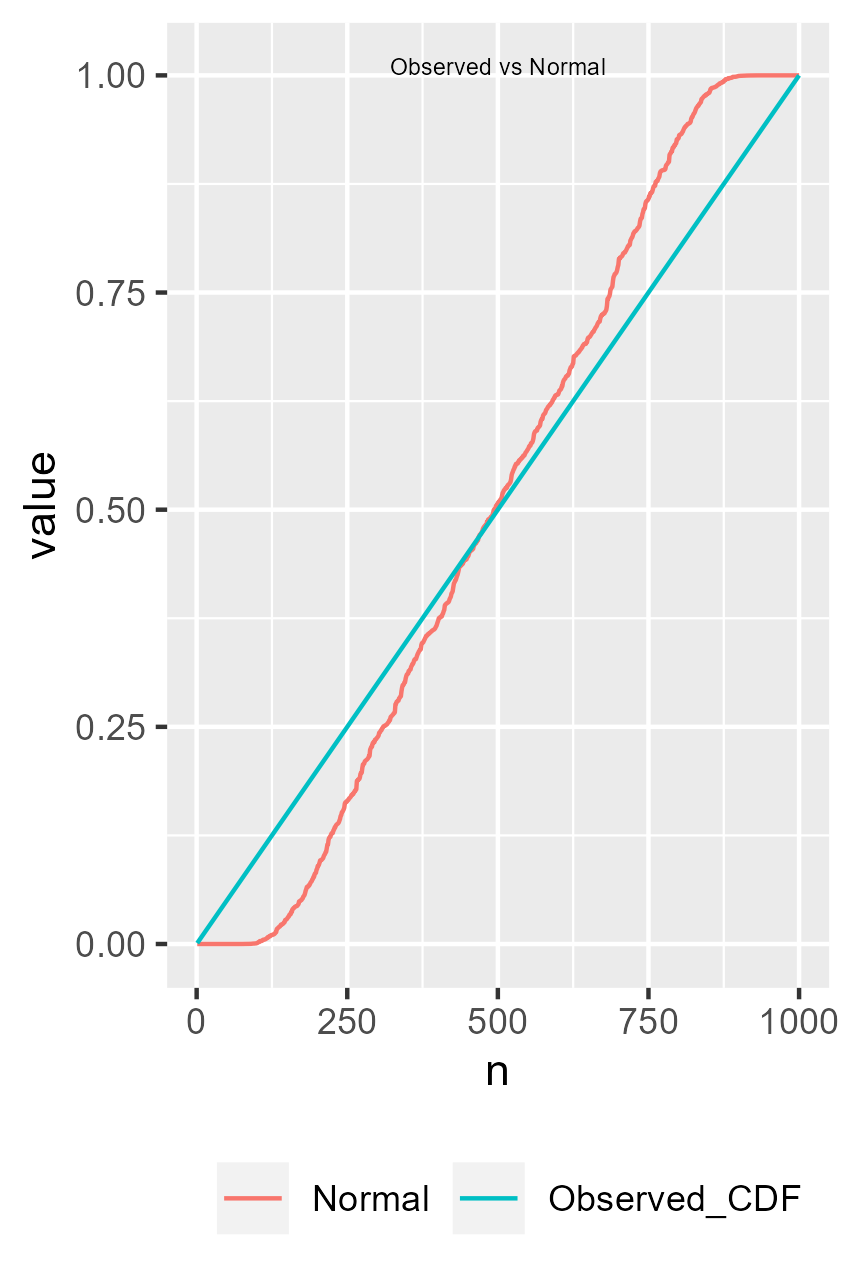
\includegraphics[width=0.7\textwidth]{graphics/kolmogorov_smirnov.png}
	  \caption{Observed and model (Normal) data}
	  \label{fig:ks:data}
	\end{figure}
%	\clearpage
\end{comment}

	A hypothesis test was carried out using results from the \texttt{kolmogorov\_smirnov}, function:

	\begin{lstlisting}[language=R]
		ks_results <-kolmogorov_smirnov(data)
		# print(ks_results)
		# A tibble: 1 x 5
		      D  Dmax   Dmin     K     pval
  		<dbl> <dbl>  <dbl> <dbl>    <dbl>
		1 0.135 0.124 -0.135  4.26 2.22e-16
	\end{lstlisting}

	\subsection*{Hypothesis Test}

	\begin{enumerate}
		\item $H_0$ the observed data is normally distributed
		%$N(\mu=\bar{x}, \sigma = sd)$
		\item $H_a$ the observed data is not normally distributed
		\item the test statistic $D$ is 0.135
		\item the $\alpha$ value is 0.05
		\item the critical value $K$ is 4.26
		\item the \texttt{pvalue} is $2.22 \times 10^{-16}$ (ie the probability of observing these values if the data was normally distributed is approximately 0)
		\item as \texttt{pvalue} is less than $\alpha$ we \textbf{reject} the null hypothesis
		($D_{\alpha,N}=0.04301$, we reject $H_\alpha$ if $D > D_{\alpha,N}$)\footnote{https://www.itl.nist.gov/div898/handbook/eda/section3/eda35g.htm}
	\end{enumerate}

	There is insufficient evidence to support the hypothesis that our observed data is normally distributed.

  The results are summarised in Table~\ref{tab:ks:results}.

	The results were checked using the \texttt{cont\_ks\_test} function from the \texttt{KSgeneral} package, and the same results were obtained.\footnote{these agreed with the results with the default \texttt{ks.test} function.}
  \begin{lstlisting}
		# KSgeneral::cont_ks_test(data, "pnorm")

			One-sample Kolmogorov-Smirnov test

		data:  data
		D = 0.13573, p-value < 2.2e-16
		alternative hypothesis: two-sided
\end{lstlisting}

%  
% Table created by stargazer v.5.2.3 by Marek Hlavac, Social Policy Institute. E-mail: marek.hlavac at gmail.com
% Date and time: Tue, Feb 07, 2023 - 18:30:59
\begin{table}[!htbp] \centering 
  \caption{Kolmogorov-Smirnov Test results - one sample} 
  \label{tab:ks:results} 
\begin{tabular}{@{\extracolsep{5pt}} cc} 
\\[-1.8ex]\hline 
\hline \\[-1.8ex] 
 & 1 \\ 
\hline \\[-1.8ex] 
Dval & $0.13473$ \\ 
Dmax & $0.12356$ \\ 
Dmin & $$-$0.13473$ \\ 
Kval & $4.26048$ \\ 
pval & $0$ \\ 
k\_alpha & $0.04301$ \\ 
\hline \\[-1.8ex] 
\end{tabular} 
\end{table} 

	\clearpage

%# Fri Feb 10 18:04:12 2023 ------------------------------

\section*{Question 2}
\noindent Estimate an OLS regression in \texttt{R} that uses the Newton-Raphson algorithm (specifically \texttt{BFGS}, which is a quasi-Newton method), and show that you get the equivalent results to using \texttt{lm}. Use the code below to create your data.
%\vspace{.5cm}

	The data was generated as follows:

	\begin{lstlisting}
		set.seed (123)
		data2 <- data.frame(x = runif(200, 1, 10))
		data2$y <- 0 + 2.75*data2$x + rnorm(200, 0, 1.5)

	\end{lstlisting}

  \begin{figure}[!htbp]
	  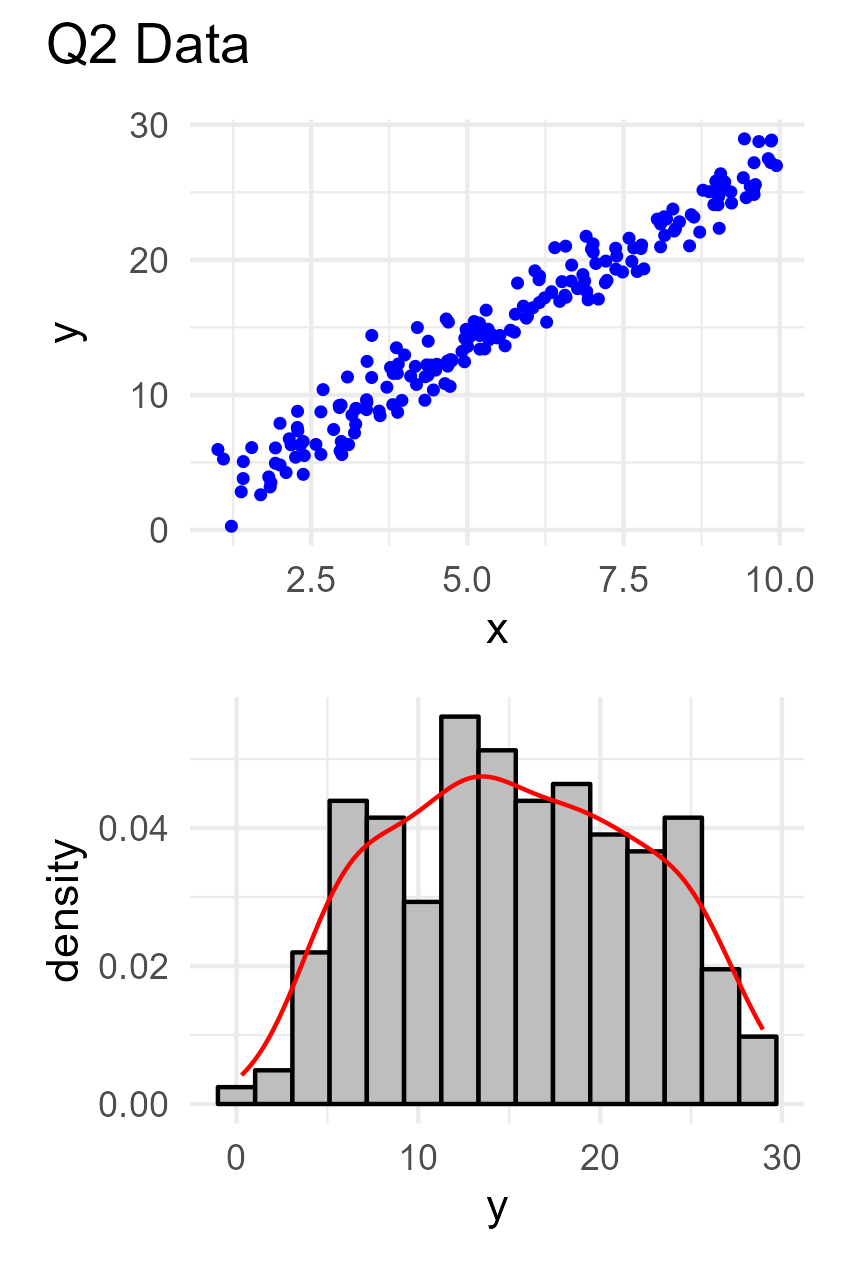
\includegraphics[width=0.75\textwidth]{graphics/q2_data.png}
	  \caption{Q2 Data}
	  \label{fig:mle:data}
	\end{figure}

\begin{comment}
  \begin{figure}[!htbp]
	  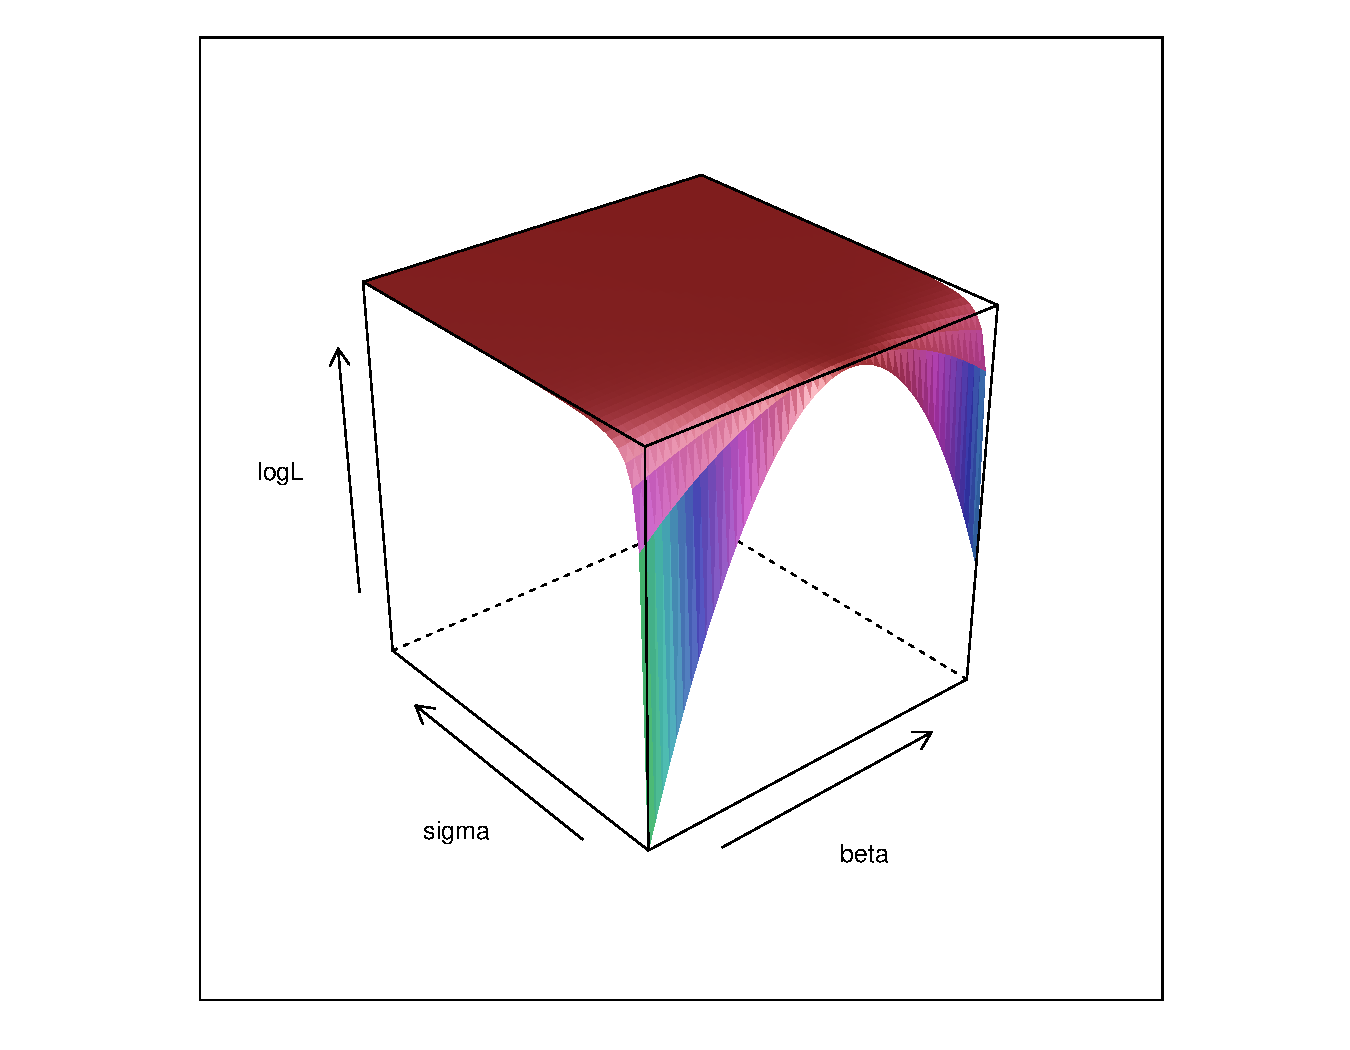
\includegraphics[width=0.7\textwidth]{graphics/wireframe.pdf}
	  \caption{mle surface}
	  \label{fig:surface}
	\end{figure}
  \begin{figure}[!htbp]
	  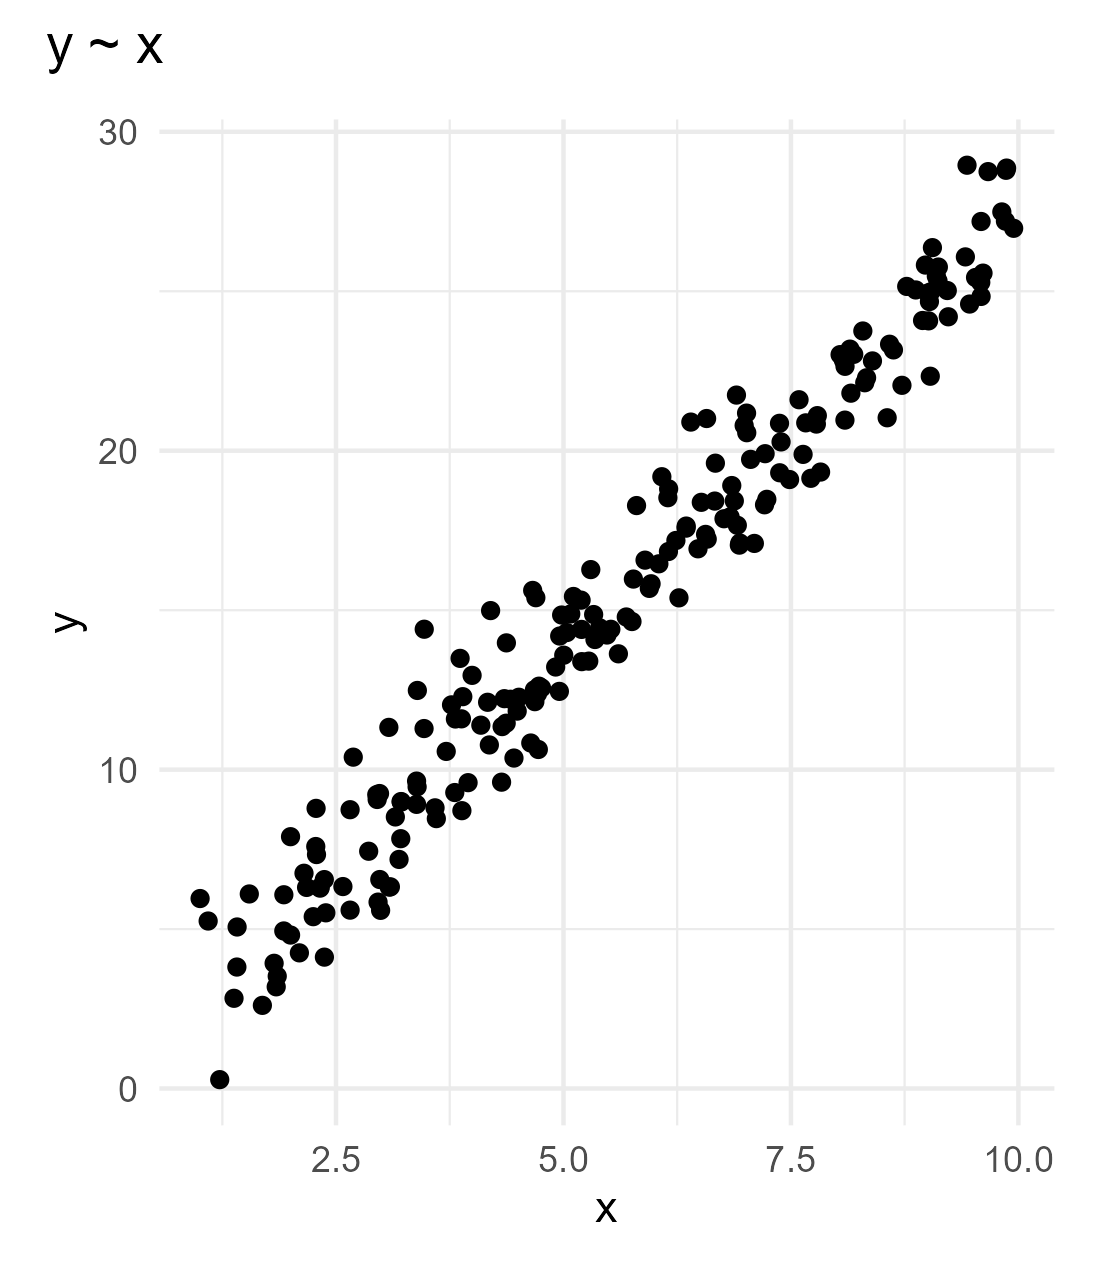
\includegraphics[width=0.7\textwidth]{graphics/q2_xy.png}
	  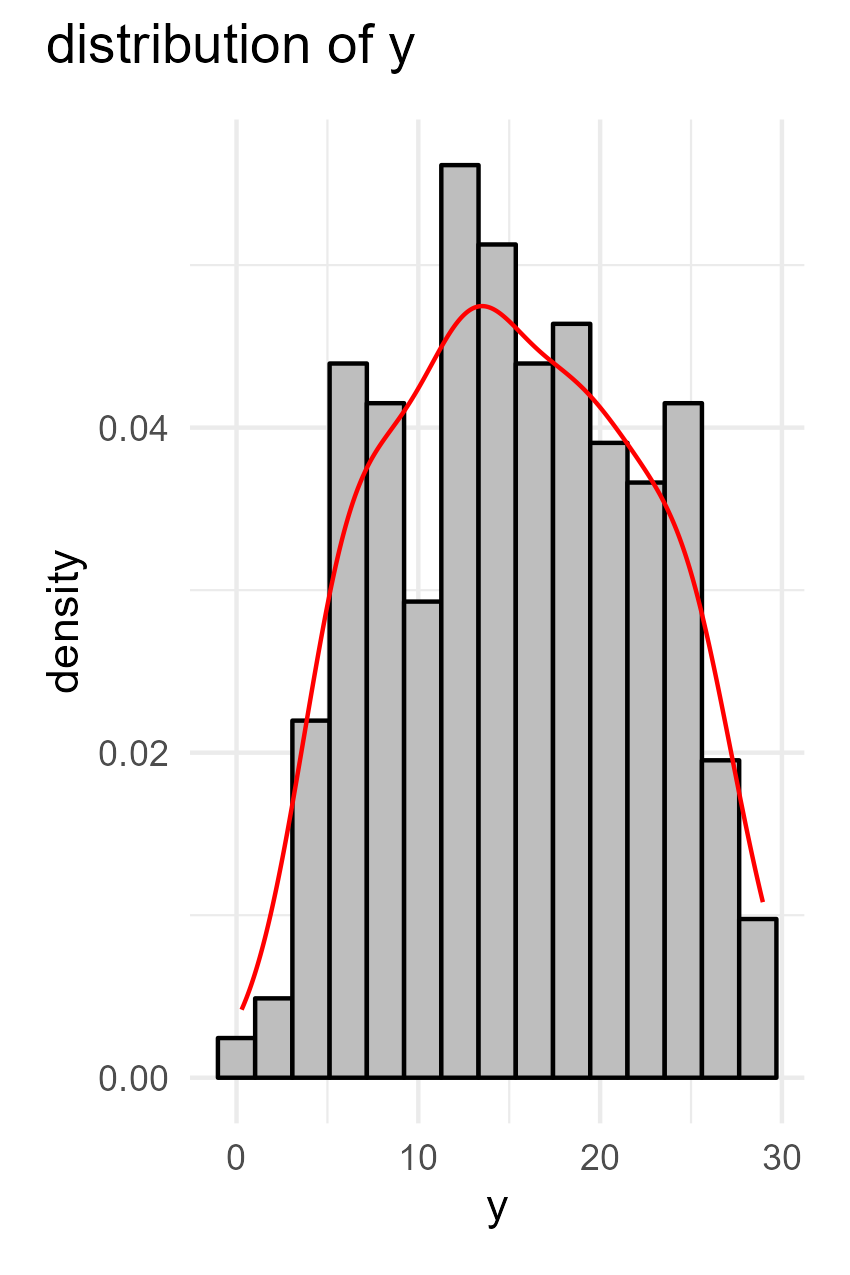
\includegraphics[width=0.7\textwidth]{graphics/q2_hist.png}
	  \caption{Q2 Data}
	  \label{fig:mle}
	\end{figure}
\end{comment}

	\clearpage

	The code to implement the {\huge Maximum Likelihood Estimation/OLS} is:
\lstinputlisting[language=R, firstline=270,lastline=288]{PS1_ImeldaFinn.R}

	\begin{lstlisting}
		linear.MLE$par
		#theta          y          X
		#0.1398324  2.7265559 -1.4390716

		linear.MLE$se
		#     theta          y          X
		#0.25140690 0.04136606 0.07191798
	\end{lstlisting}

	The linear regression model was called:

\lstinputlisting[language=R, firstline=303,lastline=303]{PS1_ImeldaFinn.R}


	The results for the MLE and linear models are in Table~\ref{tab:mle}:

% Table created by stargazer v.5.2.3 by Marek Hlavac, Social Policy Institute. E-mail: marek.hlavac at gmail.com
% Date and time: Fri, Feb 10, 2023 - 23:04:42
\begin{table}[!htbp] \centering
  \caption{}
  \label{tab:mle}
\begin{tabular}{@{\extracolsep{5pt}}lcc}
\\[-1.8ex]\hline
\hline \\[-1.8ex]
 & \multicolumn{2}{c}{\textit{Dependent variable:}} \\
\cline{2-3}
\\[-1.8ex] & \multicolumn{2}{c}{y} \\
\\[-1.8ex] & MLE & Linear\\
\hline \\[-1.8ex]
 theta & 0.1398324 &  \\
  & (0.251) &  \\
  & & \\
 y & 2.7265559 &  \\
  & (0.041) &  \\
  & & \\
 X & -1.4390716 &  \\
  & (0.072) &  \\
  & & \\
 x &  & 2.727$^{***}$ \\
  &  & (0.042) \\
  & & \\
 Constant &  & 0.139 \\
  &  & (0.253) \\
  & & \\
\hline \\[-1.8ex]
Observations & 200 & 200 \\
R$^{2}$ &  & 0.956 \\
Adjusted R$^{2}$ &  & 0.956 \\
Residual Std. Error (df = 198) &  & 1.447 \\
F Statistic &  & 4,298.687$^{***}$ (df = 1; 198) \\
\hline
\hline \\[-1.8ex]
\textit{Note:}  & \multicolumn{2}{r}{$^{*}$p$<$0.1; $^{**}$p$<$0.05; $^{***}$p$<$0.01} \\
\end{tabular}
\end{table}


	The prediction equation is: $y = 0.1398324 + 2.7265559 \times x$.

	$\hat y =  0.13983  (\theta)  +  5.55753  (\bar{x}) *  2.72656  (\beta) =  15.29274$

	$\bar y = 15.29289$








\end{document}
